

\begin{figure}
    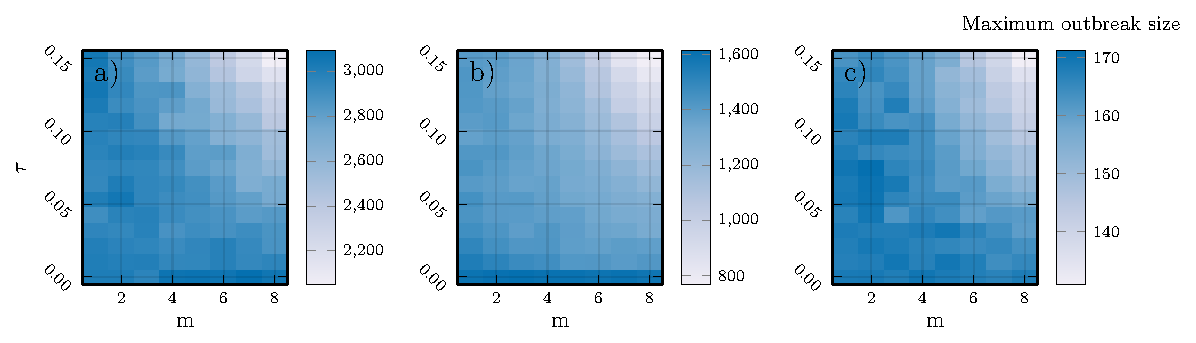
\includegraphics[width=\textwidth]{appendices/data_base_fig.pdf}
    \caption{Maximum MPB infestation size within 500 year period, under FTP with respect to $\tau$ fraction of $m$ juvenile stands cleared. a) ($\alpha_1 = 0.02$, $\alpha_2 = 0.0025$), b) ($\alpha_1 = 0.01$, $\alpha_2 = 0.006$.), c)($\alpha_1 = 0.03$, $\alpha_2 = 0.0012$.)}
    \label{beetle_pop_yearly}
  \end{figure}
  
  \begin{figure}
    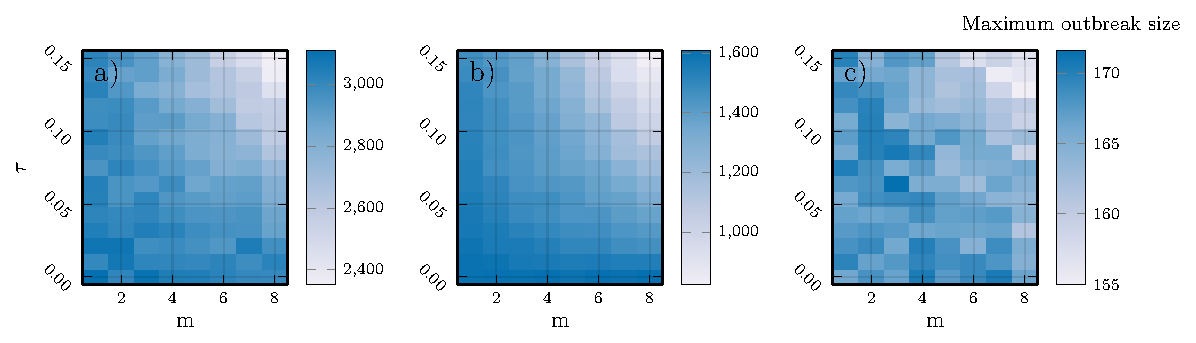
\includegraphics[width=\textwidth]{appendices/data_five_year_trim_fig.pdf}
    \caption{Maximum MPB infestation size within 500 year period, under FTP with respect to $\tau$ fraction of $m$ juvenile stands cleared, conducted every \emph{five} years. a)($\alpha_1 = 0.02$, $\alpha_2 = 0.0025$), b)($\alpha_1 = 0.01$, $\alpha_2 = 0.006$.), c)($\alpha_1 = 0.03$, $\alpha_2 = 0.0012$.)}
  \end{figure}
  
  \begin{figure}
    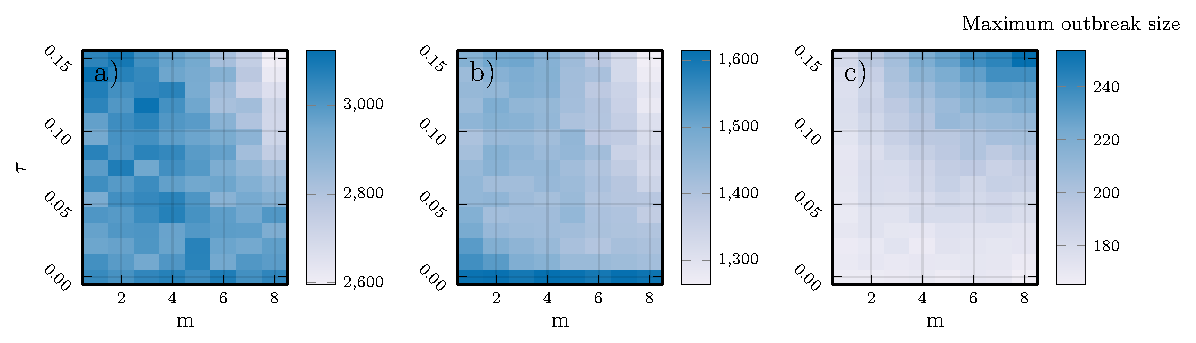
\includegraphics[width=\textwidth]{appendices/data_yearly_burn_fig.pdf}
    \caption{Maximum MPB infestation size within 500 year period, under CBP with respect to $\tau$ fraction of $m$ juvenile stands cleared, conducted each year. a)($\alpha_1 = 0.02$, $\alpha_2 = 0.0025$), b) ($\alpha_1 = 0.01$, $\alpha_2 = 0.006$.), c) ($\alpha_1 = 0.03$, $\alpha_2 = 0.0012$.)}
  \end{figure}

